\newpage

\section{Theory}
\label{sec:theory}


\subsection{Governing equations}
\label{subsec:governing_equations}
The full compressible potential equation, which is a second-order partial differential equation, can be expressed in terms of the velocity potential $\phi$ as follows:
\begin{equation}
	(1 - M^2\phi_x^2)\phi_{xx} - 2M^2\phi_x\phi_y\phi_{xy} + (1 - M^2\phi_y^2)\phi_{yy} + \phi_{zz} = 0,
\end{equation}
\label{eq:governing_equations}
where $M$ is the Mach number, and $\phi_x$, $\phi_y$, and $\phi_z$ are the partial derivatives of the velocity potential with respect to the spatial coordinates $x$, $y$, and $z$, respectively. The subscripts denote partial differentiation.

\subsection{Hypothesis}
\label{subsec:hypothesis}

\begin{itemize}
\item Inviscid, adiabatic, perfect-gas flow, steady
	\begin{equation*}
		P = \rho R T \quad ; \quad \gamma = const \quad ; \quad div(v) = 0 \quad ; \quad \frac{\partial }{\partial t} = 0
	\end{equation*}

\item Small perturbations of the flow field
	\begin{equation*}
		v = v_0 + v' \quad ; \quad P = P_0 + P' \quad ; \quad T = T_0 + T'
	\end{equation*}

\item Disturbance velocities
	\begin{equation*}
		v' = \epsilon v_1 + \epsilon^2 v_2 + \epsilon^3 v_3 + ... \quad ; \quad \epsilon << 1
	\end{equation*}

\end{itemize}

\subsection{Linearized equations}
\label{subsec:linearized_equations}
The linearized equations are obtained by substituting the perturbation velocities into the governing equations and neglecting higher-order terms. The resulting equations can be expressed as follows:
\begin{equation}
	(1 - M_\infty^2) \phi_{xx} + \phi_{yy} + \phi_{zz} = 0.
	\label{eq:small-disturb}
\end{equation}
	
This limited development neglects all terms of order \(O(\phi_x^2)\) and above, as well as shock-shock interactions, thereby restricting valid Mach and deflection ranges.

\subsection{Shock angle}
The exact oblique-shock relation for a wedge half-angle \(\theta\) is
\begin{equation}
	tan\theta = 2\cot\beta\frac{M_\infty^2\sin^2\beta - 1}{M_\infty^2(\gamma+\cos2\beta)+2}.
\end{equation}
In the limit \(\theta\to0\) with attached flow, the critical condition arises when the numerator vanishes:
\begin{equation*}
	M_\infty^2\sin^2\beta_d - 1 = 0
	\quad\Longrightarrow\quad
	\beta_d = \sin^{-1}(1/M_\infty).
\end{equation*}
So,
\begin{equation}
\beta_d \approx \sin^{-1}\Bigl(\frac{1}{M_\infty}\Bigr)
\label{eq:beta_d}
\end{equation}
offers a first-order shock-detachment estimate.  Note the distinction from the Mach angle \(\mu=\sin^{-1}(1/M_\infty)\), which applies to infinitesimal disturbances rather than finite shocks.







\subsection{Applicaiton of the theory}


\begin{center}
	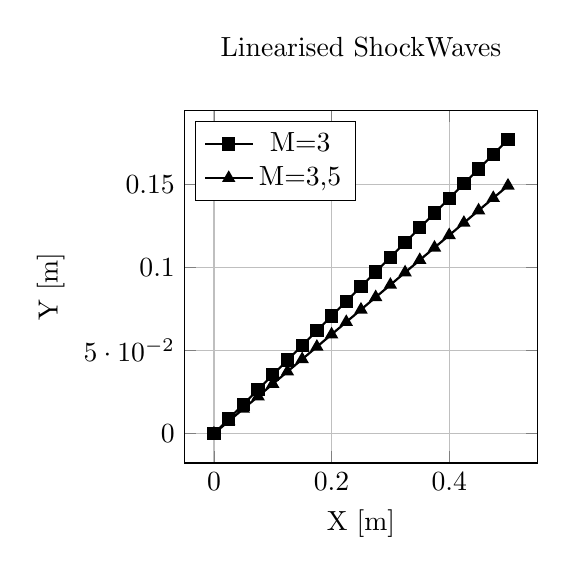
\begin{tikzpicture}
	  \begin{axis}[
		width=0.5\textwidth,
		height=0.5\textwidth,
		xlabel={X [m]},
		ylabel={Y [m]},
		title={Linearised ShockWaves},
		title style={yshift=10pt},
		grid=major,
		legend style={legend pos=north west},
		% scaled x ticks=false,  % éventuellement pour afficher en pleine valeur
	  ]
		\addplot[
		  smooth,
		  mark=square*,
		  thick,
		] coordinates {
			(0, 0)
			(0.025, 0.008838835)
			(0.05, 0.01767767)
			(0.075, 0.026516504)
			(0.1, 0.035355339)
			(0.125, 0.044194174)
			(0.15, 0.053033009)
			(0.175, 0.061871843)
			(0.2, 0.070710678)
			(0.225, 0.079549513)
			(0.25, 0.088388348)
			(0.275, 0.097227182)
			(0.3, 0.106066017)
			(0.325, 0.114904852)
			(0.35, 0.123743687)
			(0.375, 0.132582521)
			(0.4, 0.141421356)
			(0.425, 0.150260191)
			(0.45, 0.159099026)
			(0.475, 0.167937861)
			(0.5, 0.176776695)		
		};
		\addlegendentry{M=3};
	
		\addplot[
		  smooth,
		  mark=triangle*,
		  thick,
		] coordinates {
			(0, 0)
			(0.025, 0.00745356)
			(0.05, 0.01490712)
			(0.075, 0.02236068)
			(0.1, 0.02981424)
			(0.125, 0.0372678)
			(0.15, 0.04472136)
			(0.175, 0.052174919)
			(0.2, 0.059628479)
			(0.225, 0.067082039)
			(0.25, 0.074535599)
			(0.275, 0.081989159)
			(0.3, 0.089442719)
			(0.325, 0.096896279)
			(0.35, 0.104349839)
			(0.375, 0.111803399)
			(0.4, 0.119256959)
			(0.425, 0.126710519)
			(0.45, 0.134164079)
			(0.475, 0.141617639)
			(0.5, 0.149071198)
		};
		\addlegendentry{M=3,5};
	
	  \end{axis}
	\end{tikzpicture}
\end{center}